\chapter{Implementácia}

\section{Implementácia neurónových sietí}
Pre potreby merania pamäťovej hĺbky sme potrebovali 
veľmi modifikované implementácie neurónových sietí, 
preto sme sa rozhodli pre ich vlastnú implementáciu. 
Vlastná implementácia nám umožnila experimentovať s rôznymi typmi kontextov a rôznymi spôsobmi 
trénovania sietí, čo s existujúcimi implementáciami bolo veľmi nepraktické a v istých prípadoch nemožné.
Medzi špeciálne prípady patrí napríklad použitie modifikovaných kontextov, 
úprava excitačnej funkcie počas trénovania (zmenšovanie okolia), dynamické znižovanie rýchlosti
učenia siete počas trénovania/po jednotlivých epochách trénovania, vytvorenie pamäťového okna v jednotlivých neurónoch 
a samotné meranie pamäťovej hĺbky.

\section{Voľba programovacieho jazyka}
Ako implementačný jazyk sme zvolili Python pretože preň existuje veľké množstvo kvalitných knižníc pre prácu
s maticami a vektormi, či vykresľovanie grafov.
Python je veľmi populárny v oblasti strojového učenia. 
Ďaľšou výhodou je jednoduché spustenie skriptov
na linuxovom serveri, čo urýchľuje samotné trénovanie a hľadanie optimálnych parametrov a umožnilo nám otestovať 
veľké množstvo kombinácii rôznych parametrov.
\subsection{Python}

Python je interpretovaný vysokoúrovňový programovací jazyk. 
Python kladie dôraz na jednoduchosť a čitateľnosť programov, ktoré sú v ňom naprogramované.
Je to jazyk, ktorý využíva dynamické typovanie a automatizovanú správu pamäte. Je to tiež multiplatformový 
jazyk a beží na všetkých bežne používaných platformách (Windows, Mac, Linux)

\section{Použité knižnice a softvér}
Používame štandartný set knižníc pre implementáciu neurónových sietí: numpy, scipy.
Na vykresľovanie a vizualizáciu dát používame knižnice matplotlib a seaborn.
\subsection{Numpy}
Je knižnica, ktorá uľahčuje prácu s maticami, používaná je takmer všetkými existujúcimi
knižnicami, ktoré implementujú modely strojového učenia v Pythone. Má vysokú úroveň optimalizácie
a požíva veľmi optimalizované funkcie na prácu s maticami, ktoré sú naprogramované v jazyku C.
\subsection{Matplotlib}
Je knižnica na vykresľovanie grafov a vizualizáciu dát.
\subsection{Seaborn}
Je nadstavbou Matplotlib knižnice a zjednodušuje vykresľovanie rôznych grafov.
\subsection{MultiDendrograms}
Jednoduchý java program, ktorý slúži na vykresľovanie dendrogramov z podobnostných matíc. 
Autorom je Sergio Gómez. V našej práci ho používame pri experimente s SRN sieťou na vizualizáciu
súvislostí medzi vstupmi.
\url{http://deim.urv.cat/~sergio.gomez/multidendrograms.php}


\section{Algoritmus hľadania najdlhšej spoločnej postfixovej podpostupnosti viacerých reťazcov}
Na hľadanie najdlhšej spoločnej podpostupnosti viacerých reťazcov som použil relatívne jednoduchý algoritmux.
Na začiatku si inicializujeme veľkosť najdlhšej spoločnej podpostupnosti na nulu.
V cykle prechádzame postupne všetky posuvné okná uložené v pamäťovom okne neurónu a kontrolujeme
či sú znaky na i-tej pozícii od konca rovnaké. Ak áno inkrementujeme veľkosť najdlhšej spoločnej podpostupnosti.
Ak nie, tak skončíme a vrátime veľkosť najdlhšej spoločnej podpostupnosti.
V prípade, že pamäťové okno neurónu obsahuje iba jednu podpostupnosť, potom dĺžka najdlhšej podpostupnosti je 
rovná dĺžke uloženého posuvného okna. V prípade ak je pamäťové okno neurónu prázdne, dĺžka najdlhšej spoločnej
podpostupnosti je nulová.
Tento algoritmus je jednoduchý a dostatočne efektívny pre meranie pamäťovej hĺbky testovaných sietí. 
Na rýchlosť trénovania má výpočet pamäťovej hĺbky iba minimálny vplyv.

\section{Reberov automat}
Na vytvorenie trénovacej množiny, ktorá pozotáva z reberových reťazcov sme si vytvorili vlastnú implementáciu pravdepodobnostného nedeterministického
konečného reberového automatu, pomocou ktorého generujeme reberové reťazce.
Každý stav okrem počiatočného a konečného stavu má práve dva prechody do ďaľšieho stavu, 
pričom v každom stave je 50\% šanca na prechod do jedného z možných stavov.
\begin{figure}[H]
    \centering
    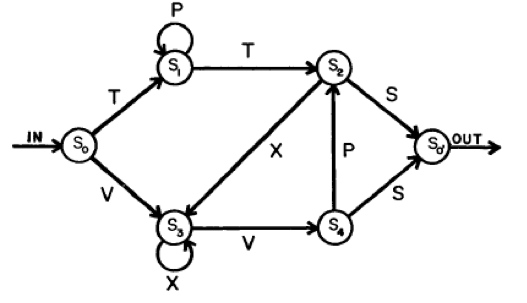
\includegraphics[width=8cm]{assets/reber}
    \caption{Schéma reberovho automatu, Zdroj:\url{http://www.replicatedtypo.com/cultural-inheritance-in-studies-of-artifical-grammar-learning/3352.html}}
\end{figure}

\section{Zdrojové kódy}
Kompletné zdrojové kódy implementovaných neurónových sietí a výsledky je možno nájsť na githube \url{https://github.com/jaroslavistok/NeuralNetsMemorySpan}.
